\documentclass[11pt,a4paper]{report}

\usepackage{graphicx}
\usepackage{epstopdf}
\usepackage[section]{placeins} % 'one-shot' command to nicely place figures
\usepackage{datatool}
\usepackage{url}
\DeclareUrlCommand\UScore{\urlstyle{rm}}



\newcommand{\anuga}{\textsc{anuga}}


\newcommand{\inputresults}[1]{\graphicspath{{#1/}}
\section{Dam Break}

Standard dam break test problem. Should show rarefaction fan and shock. 

\subsection{Results}


We should see excellent agreement between the analytical and numerical solutions.

\begin{figure}[h]
\begin{center}
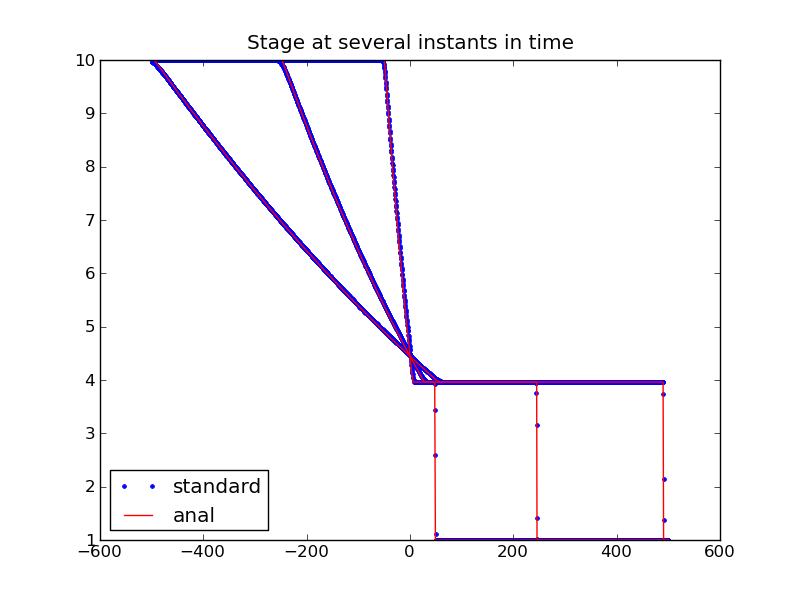
\includegraphics[width=0.9\textwidth]{stage_plot.png}
\end{center}
\caption{Stage results}
\end{figure}


\begin{figure}[h]
\begin{center}
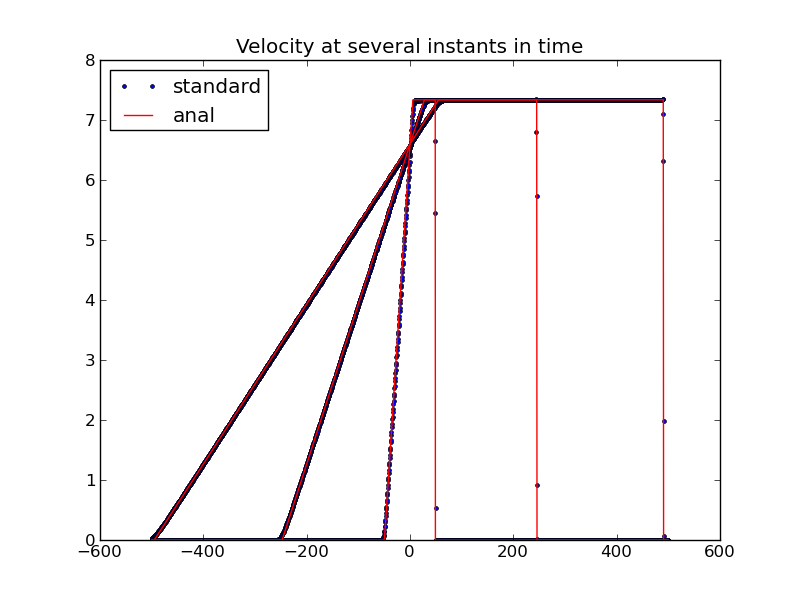
\includegraphics[width=0.9\textwidth]{xvel_plot.png}
\end{center}
\caption{Velocity results}
\end{figure}


\endinput
}
\newcommand{\cfl}{\UScore{1.0}}
\newcommand{\alg}{\UScore{tsunami}}
\newcommand{\majorR}{\UScore{1.3.0_beta}}
\newcommand{\minorR}{\UScore{8581}}
\newcommand{\timeR}{{Tue Sep 18 15:39:06 2012}}


%=========================================
\begin{document} 
%=========================================

\title{Automated Report on the Performance of \anuga{} on Various Test Problems}
\maketitle
\tableofcontents

%======================
\chapter{Introduction}
%======================

The results in this report were produced by \anuga{} version \majorR{} 
from svn repository revision \minorR{} at time \timeR.
The flow algorithm was \alg{} and CFL condition \cfl.

%======================
\chapter{Simple Tests}
%======================

\inputresults{Tests/Analytical_exact/dam_break_dry}

%\inputresults{Tests/Simple/runup1}

%\inputresults{Tests/Simple/runup_sinusoid}

%\inputresults{Tests/Simple/trapezoidal_channel}

%\inputresults{Tests/Simple/parabolic_basin_1D}

%\inputresults{Tests/Simple/deep_wave}

%\inputresults{Tests/Simple/steep_slope}

%%======================
%\chapter{Benchmark Tests}
%%======================

%\inputresults{Tests/Benchmarks/Isolated_Building}

%\inputresults{Tests/Benchmarks/Okushiri}

%======================
%\chapter{Real World Tests}
%======================

%\inputresults{Tests/Real_World/Patong}

%======================
\appendix
%======================
%======================
\chapter{Adding New Tests}
%======================


To setup a new validation test, create a test directory under the
\textsc{Tests} directory. In that directory there should be the test code, a
\TeX{} file \texttt{results.tex} and a python script
\texttt{produce\_results.py}, which runs the simulation and produces the
outputs. Copy the format from the other test directory. 

In this \TeX{} file, \texttt{report.tex}, add a line
\begin{verbatim}
\inputresults{Tests/Directory/Name}
\end{verbatim}



\section{Algorithm Parameters}
Parameters can be communicated from the \verb|parameters.py|
file in the \verb|validation_tests| directory.

In particular the
values of \verb|alg| (flow algorithm) and \verb|cfl| (CFL Condition)
are passed as command options when calling \verb|produce_results.py| in the
test directories.

You can pass though the parameters straight from the \verb|parameters.py| file as follows
\begin{verbatim}
from validation_tests.parameters import alg
from validation_tests.parameters import cfl
\end{verbatim}

\section{Generic form of \texttt{produce\_results.py}}

The \texttt{produce\_results.py} files in the test directories should have the
following general form

\begin{verbatim}
from fabricate import *
from validation_tests.utilities import run_validation_script

# Setup the python scripts which produce the output for this
# validation test
def build():
    run_validation_script('run_problem.py')
    run_validation_script('plot_problem.py')
    pass

def clean():
    autoclean()

main()
\end{verbatim}
This script uses \texttt{fabricate} which automatically determines dependences
and only runs the command if the parameters alg and cfl have changed,
or input/output or source files have changed. (\texttt{fabricate} is a replacement for
standard \texttt{make})


%======================
% bibliography
%======================

\bibliographystyle{plain}
\bibliography{bibliography}

\end{document}
